\chapter{Ising Correlations, Mean Field, and Spontaneous Magnetization}

\lectureoverview{A one-dimensional Ising chain can be solved exactly by replacing site spins with bond variables. That change of variables turns the partition function into a product and shows that every finite-temperature correlation decays exponentially. Higher-dimensional lattices behave differently because each spin receives information from many neighbors. Treating their combined influence as an average field gives a self-consistency equation, a mean-field critical temperature, and a precise account of how an arbitrarily small external field selects one magnetized phase.}

\section{What Ising Actually Found}

The historical point should be stated accurately. Ernst Ising solved the one-dimensional model assigned by Wilhelm Lenz and correctly found no finite-temperature phase transition. The overreach was the inference that the same conclusion should hold in every dimension. It does not. The two-dimensional model already has an ordered low-temperature phase.

An exact solution in higher dimension is too ambitious for the present purpose. A physically transparent approximation will be enough to expose the transition when each spin has many neighbors. Before making that approximation, however, it is worth solving the one-dimensional chain exactly. The contrast between the exact one-dimensional answer and the high-dimensional approximation identifies the mechanism that one dimension lacks.

A phase transition here means more than a gradual strengthening of an existing preference. As temperature crosses a critical value, the equilibrium state acquires a new macroscopic property: a nonzero magnetization can persist even after the external field used to orient the sample has been removed. The calculation must therefore answer two separate questions. Does a distant spin remember the orientation of a chosen spin, and can an infinitesimal field organize an arbitrarily large sample?

\section{One Spin as the Reusable Building Block}

Take a two-state variable
\begin{equation}
\sigma=\pm1,
\end{equation}
and choose the energy convention
\begin{equation}
E(\sigma)=-J\sigma,
\qquad J>0.
\end{equation}
The state \(\sigma=+1\) then has lower energy. The parameter \(J\) may stand for a magnetic moment multiplied by an applied field, but only the product enters this calculation.

Treat this spin as a small subsystem in thermal equilibrium with everything else. Its partition function is
\begin{align}
z
&=\sum_{\sigma=\pm1}e^{-\beta E(\sigma)}
 =\sum_{\sigma=\pm1}e^{\beta J\sigma} \\
&=e^{\beta J}+e^{-\beta J}
 =2\cosh(\beta J).
\end{align}

The same result could be embedded in a collection of \(N\) independent spins. The full partition function would simply be \(Z=z^N\), so \(\log Z=N\log z\) and every extensive thermodynamic quantity would be \(N\) times its one-spin value. This subsystem viewpoint replaces the longer combinatorial count of how many spins point up and down, but it contains the same information.
The average energy follows from the logarithmic derivative:
\begin{align}
\expect{E}
&=-\frac{\partial}{\partial\beta}\log z \\
&=-J\frac{\sinh(\beta J)}{\cosh(\beta J)}
 =-J\tanh(\beta J).
\end{align}
Since \(E=-J\sigma\),
\begin{equation}
\expect{\sigma}=\tanh(\beta J).
\end{equation}

\begin{figure}[ht]
\centering

\includegraphics[width=0.80\textwidth]{lecture_09_figure_02.png}
\caption{The one-spin energy and magnetization reduced to hyperbolic-tangent form.}
\lectureframe{00:10:06}
\end{figure}

This one formula contains both temperature limits. At low temperature, \(\beta J\gg1\), and the spin is almost certainly in the lower-energy state. At high temperature, \(\beta J\ll1\), so
\begin{equation}
\expect{\sigma}\simeq \beta J\longrightarrow0.
\end{equation}
Thermal agitation erases the energetic bias.

\begin{classroomqa}
\audiencequestion{Should the average energy carry a minus sign?}
\lecturerresponse{Yes. The thermodynamic identity is \(\expect{E}=-\partial_\beta\log z\), so the result is \(-J\tanh(\beta J)\). Dividing by the factor \(-J\) in \(E=-J\sigma\) then gives the positive magnetization \(\expect{\sigma}=\tanh(\beta J)\). \lecturetimestamp{00:09:15--00:09:44}}
\end{classroomqa}

\section{The One-Dimensional Chain}

Place \(N\) spins on an open chain and let neighboring spins interact:
\begin{equation}
H=-J\sum_{i=1}^{N-1}\sigma_i\sigma_{i+1},
\qquad \sigma_i=\pm1.
\label{eq:ising-chain}
\end{equation}
For \(J>0\), a parallel pair contributes \(-J\), while an antiparallel pair contributes \(+J\). The two ground states are therefore
\begin{equation}
(+,+,\ldots,+)
\qquad\text{and}\qquad
(-,-,\ldots,-).
\end{equation}

\begin{figure}[ht]
\centering

\includegraphics[width=0.80\textwidth]{lecture_09_figure_03.png}
\caption{The open-chain Hamiltonian and its Boltzmann sum.}
\lectureframe{00:19:15}
\end{figure}

Changing \(J\) to \(-J\) favors alternating spins. On an open chain, or on an even periodic chain, the redefinition
\begin{equation}
\widetilde{\sigma}_i=(-1)^i\sigma_i
\end{equation}
maps the antiferromagnetic sign back to the ferromagnetic one. The distinction is physical, but the one-dimensional partition-function algebra is the same. An odd periodic chain is the familiar exception because it cannot alternate without frustration.

\begin{classroomqa}
\audiencequestion{Is there an external magnetic field in the chain Hamiltonian?}
\lecturerresponse{Not yet. Equation~\eqref{eq:ising-chain} contains only nearest-neighbor coupling. A uniform external field will be added later as a separate term, \(-h\sum_i\sigma_i\), precisely to test how the ordered state responds to an arbitrarily small bias. \lecturetimestamp{00:18:54--00:19:13}}
\end{classroomqa}

\subsection{Memory as a correlation function}

Suppose \(\sigma_i\) is known to be up. Does that information influence a spin \(r\) bonds away? The diagnostic is
\begin{equation}
C(r)=\expect{\sigma_i\sigma_{i+r}}.
\end{equation}
If \(C(r)\) approaches a nonzero number as \(r\to\infty\), the system retains long-range memory. If it approaches zero, the effect of the first spin eventually disappears.

The game of telephone gives the right intuition. Each person transmits one binary symbol to the next. If every transmission is perfect, the initial bit survives indefinitely. If each step has any nonzero error probability, repeated transmission eventually loses the original message. Zero temperature is the perfect-transmission limit of the Ising chain. Any positive temperature permits occasional disagreements between neighbors.

For a numerical picture, suppose a single transmission has fidelity \(0.99\). Two perfect transmissions occur with probability \(0.99^2=0.9801\), and each additional step supplies another factor of \(0.99\). A hundred steps already make errors common; ten thousand steps erase practical memory. The Ising chain uses a signed measure of fidelity rather than this no-error probability, but the multiplicative loss is the same idea.

The analogy becomes exact after distinguishing a probability from a correlation. If \(p\) is the probability that adjacent spins agree, then
\begin{equation}
\expect{\sigma_i\sigma_{i+1}}
=p-(1-p)=2p-1.
\end{equation}
Thus the quantity multiplied from link to link is the excess fidelity \(2p-1\), not \(p\) itself.

\section{Bond Variables and the Exact Partition Function}

The decisive change of variables is to describe relationships rather than individual spins:
\begin{equation}
\mu_i=\sigma_i\sigma_{i+1},
\qquad i=1,\ldots,N-1.
\label{eq:bond-variable}
\end{equation}
Each bond variable is \(+1\) for agreement and \(-1\) for disagreement. If the first spin is fixed, the bonds determine every later spin:
\begin{align}
\sigma_2&=\sigma_1\mu_1,\\
\sigma_3&=\sigma_1\mu_1\mu_2,\\
\sigma_{r+1}&=\sigma_1\prod_{k=1}^{r}\mu_k.
\end{align}
There is no redundancy. The data \((\sigma_1,\mu_1,\ldots,\mu_{N-1})\) are equivalent to \((\sigma_1,\ldots,\sigma_N)\).

In these variables the energy is simply
\begin{equation}
H=-J\sum_{i=1}^{N-1}\mu_i.
\end{equation}
The interacting site variables have become independent bond variables. Summing first over the two values of \(\sigma_1\) gives
\begin{align}
Z_N
&=2\sum_{\{\mu_i=\pm1\}}
\exp\left(\beta J\sum_{i=1}^{N-1}\mu_i\right)\\
&=2\prod_{i=1}^{N-1}
\left(\sum_{\mu_i=\pm1}e^{\beta J\mu_i}\right)\\
&=2\left[2\cosh(\beta J)\right]^{N-1}.
\label{eq:chain-partition}
\end{align}
There are \(N-1\) factors because an open chain of \(N\) sites has \(N-1\) bonds.

The leading factor of two is the global choice of the first spin. It contributes only \(\log2\) to \(\log Z_N\), while the bonds contribute a term proportional to \(N-1\). The factor matters for exact finite-size counting but disappears from the free-energy density as \(N\to\infty\). This is why the board could call it "no big deal" without actually discarding it.

\begin{figure}[ht]
\centering

\includegraphics[width=0.82\textwidth]{lecture_09_figure_04.png}
\caption{The site Hamiltonian rewritten as a sum over independent bonds and the resulting factorized partition function.}
\lectureframe{00:35:35}
\end{figure}

\begin{classroomqa}
\audiencequestion{Where did the sum in the exponent go when the final answer became a power?}
\lecturerresponse{It became a product before it became a power:
\[
e^{\beta J\sum_i\mu_i}=\prod_i e^{\beta J\mu_i}.
\]
The sum over all bond configurations then separates into one two-term sum for each bond. Since every factor is \(2\cosh(\beta J)\), the product is its \((N-1)\)st power. Writing out three spins and two bonds makes the factorization completely explicit. \lecturetimestamp{00:33:25--00:35:36}}
\end{classroomqa}

This is a simple dual description: coupled variables on sites have been replaced by uncoupled variables on bonds. The word \emph{duality} is appropriate because the same system has two descriptions with very different-looking degrees of freedom. Here it is an exact change of variables for an open one-dimensional chain.

In lattice language, the original variables live on vertices and the new variables live on edges. The global first-spin choice is the one extra datum needed to reconstruct vertices from edges. This site-bond exchange is a modest example of a pattern that becomes much more powerful in higher-dimensional statistical mechanics.

\subsection{Nearest-neighbor fidelity}

Every bond has the same distribution,
\begin{equation}
\Pr(\mu=+1)=\frac{e^{\beta J}}{2\cosh(\beta J)},
\qquad
\Pr(\mu=-1)=\frac{e^{-\beta J}}{2\cosh(\beta J)}.
\end{equation}
Consequently,
\begin{equation}
\expect{\mu_i}
=\expect{\sigma_i\sigma_{i+1}}
=\tanh(\beta J).
\label{eq:nearest-correlation}
\end{equation}

\begin{figure}[ht]
\centering

\includegraphics[width=0.80\textwidth]{lecture_09_figure_05.png}
\caption{The nearest-neighbor correlation expressed as the average bond variable.}
\lectureframe{00:36:52}
\end{figure}

The probability that neighbors agree is therefore
\begin{equation}
p_{\rm same}
=\frac{1+\tanh(\beta J)}{2}.
\end{equation}
It exceeds one half at positive \(J\), approaches one at zero temperature, and becomes one half at infinite temperature.

\begin{classroomqa}
\audiencequestion{Why does a positive nearest-neighbor correlation mean that the spins prefer alignment rather than anti-alignment?}
\lecturerresponse{For \(J>0\), an aligned bond has energy \(-J\) and an anti-aligned bond has energy \(+J\). The positive value of \(\expect{\mu}\) says that \(\mu=+1\), hence alignment, occurs more often. Whether a real material has ferro- or antiferromagnetic effective coupling depends on its microscopic electronic structure; the present sign convention describes a ferromagnet. \lecturetimestamp{00:43:45--00:44:48}}
\end{classroomqa}

\begin{classroomqa}
\audiencequestion{What happens to this correlation at very high temperature?}
\lecturerresponse{As \(T\to\infty\), \(\beta\to0\) and \(\tanh(\beta J)\to0\). Then even nearest neighbors carry no information about one another: each spin is effectively a random guess. \lecturetimestamp{00:46:42--00:47:20}}
\end{classroomqa}

\subsection{Long-distance correlation}

For spins separated by \(r\) bonds,
\begin{align}
\sigma_i\sigma_{i+r}
&=\sigma_i
\left(\prod_{k=i+1}^{i+r-1}\sigma_k^2\right)
\sigma_{i+r}\\
&=(\sigma_i\sigma_{i+1})
(\sigma_{i+1}\sigma_{i+2})\cdots
(\sigma_{i+r-1}\sigma_{i+r})\\
&=\prod_{k=i}^{i+r-1}\mu_k.
\end{align}
Because the \(\mu_k\) are independent,
\begin{equation}
C(r)=\expect{\sigma_i\sigma_{i+r}}
=\left[\tanh(\beta J)\right]^r.
\label{eq:exact-correlation}
\end{equation}

\begin{figure}[ht]
\centering

\includegraphics[width=0.80\textwidth]{lecture_09_figure_06.png}
\caption{Intermediate factors of \(\sigma_k^2=1\) convert the distant-spin product into a product of independent bonds.}
\lectureframe{00:41:35}
\end{figure}

\begin{classroomqa}
\audiencequestion{The correlation function contains only the two endpoint spins. Where did all the intermediate spins come from?}
\lecturerresponse{They were inserted only as factors of one: \(\sigma_k^2=1\). Pairing adjacent copies converts the endpoint product into bond variables, which are exactly the variables whose thermal distribution factorizes. The value of the correlation function has not been changed. \lecturetimestamp{00:41:41--00:42:26}}
\end{classroomqa}

At every finite temperature,
\begin{equation}
0<\tanh(\beta J)<1,
\end{equation}
so memory decays exponentially. Writing
\begin{equation}
C(r)=e^{-r/\xi}
\end{equation}
defines the exact correlation length
\begin{equation}
\xi^{-1}=-\log\!\left[\tanh(\beta J)\right].
\label{eq:correlation-length}
\end{equation}
Only at \(T=0\) does \(\xi\) diverge. At low but nonzero temperature,
\begin{equation}
\xi\simeq \frac{1}{2}e^{2\beta J},
\end{equation}
so the chain can contain very long aligned stretches without possessing true infinite-range order.

The chain therefore looks clumped. One sees a long run of up spins, then a switch, then a long run of down spins, then another switch. Low temperature makes the runs long because a domain wall is rare; it does not eliminate domain walls altogether. Magnetization requires an infinite memory length, not merely a very large one.

\section{Why More Neighbors Change the Problem}

One dimension provides no error correction. Once a bond disagrees with its predecessor, the next spin has no independent source telling it which orientation was intended. The chain therefore consists of long aligned domains separated by occasional switches.

In a square lattice each site has four nearest neighbors. In a cubic lattice it has six. On a \(d\)-dimensional hypercubic lattice it has
\begin{equation}
z=2d
\end{equation}
nearest neighbors. A site receiving three agreeing messages and one disagreeing message can follow the majority. The many-neighbor environment suppresses isolated errors in much the same way that redundant messages enable error correction.

If the neighbors have mean spin \(m\), their sum has mean \(zm\). Its ordinary fluctuation is of order \(\sqrt{z}\), so away from \(m=0\) the relative fluctuation scales approximately as
\begin{equation}
\frac{\sqrt{z}}{z|m|}
=\frac{1}{\sqrt{z}\,|m|}.
\end{equation}
This is why an average field becomes plausible at large coordination number. It also warns us that the approximation becomes least reliable near a critical point, where \(m\) is small.

A remembered saying captures the large-number intuition: a hundred independent votes are unlikely to be wrong in the same direction. The quantitative version is the square-root law. A coherent bias in \(z\) variables is proportional to \(z\), while random disagreement is typically proportional only to \(\sqrt{z}\). Increasing dimension therefore changes not only the number of neighbors but the reliability of their collective message.

\begin{classroomqa}
\audiencequestion{Do dimensions higher than three correspond to a physical magnetic material?}
\lecturerresponse{Not directly as spatial dimensions. Large \(d\) is a solvable limit in which each site has many neighbors and averaging becomes controlled. Once the mechanism is visible there, one can ask how far toward the physical dimensions it survives. For the Ising model, two dimensions are already enough for a finite-temperature transition, although mean field does not give the exact two-dimensional answer. \lecturetimestamp{00:52:32--00:53:50}}
\end{classroomqa}

\section{Mean Field as a Self-Consistency Problem}

Focus on one spin \(\sigma_i\). Its interaction with its \(z=2d\) neighbors is
\begin{equation}
E_i=-J\sigma_i\sum_{j\in{\rm nn}(i)}\sigma_j.
\label{eq:local-energy}
\end{equation}
Let
\begin{equation}
m=\expect{\sigma}
\end{equation}
denote the uniform magnetization per spin. Mean field replaces the fluctuating neighbor sum by its average:
\begin{equation}
\sum_{j\in{\rm nn}(i)}\sigma_j
\longrightarrow zm=2dm.
\end{equation}
The distinguished spin then has the effective one-spin energy
\begin{equation}
E_i^{\rm MF}=-2dJm\,\sigma_i.
\label{eq:mean-field-energy}
\end{equation}

\begin{figure}[ht]
\centering

\includegraphics[width=0.82\textwidth]{lecture_09_figure_07.png}
\caption{A selected spin, its \(2d\) nearest neighbors, and the replacement of their sum by the average magnetization.}
\lectureframe{01:00:30}
\end{figure}

The one-spin result can now be reused with the effective field \(2dJm\):
\begin{equation}
\expect{\sigma_i}_{\rm effective}
=\tanh(2\beta dJm).
\end{equation}
But the selected site is not special. Translation invariance requires its average to equal the assumed average \(m\). Hence
\begin{equation}
\boxed{m=\tanh(2\beta dJm)}.
\label{eq:self-consistency}
\end{equation}
This is why mean field is also called the self-consistent-field approximation: the magnetization that creates the effective field must equal the magnetization produced by that field.

\begin{classroomqa}
\audiencequestion{Is a factor of \(\beta\) missing from the effective one-spin answer?}
\lecturerresponse{It must be present. The argument of an exponential or a hyperbolic tangent is dimensionless, so the effective energy \(2dJm\) appears as \(2\beta dJm\). \lecturetimestamp{01:00:13--01:00:27}}
\end{classroomqa}

\begin{classroomqa}
\audiencequestion{Does the equation merely say that \(m\) is proportional to itself?}
\lecturerresponse{No. The unknown magnetization occurs inside a nonlinear function:
\[
m=\tanh(2\beta dJm).
\]
It is an implicit equation and may possess one or several solutions, depending on temperature. \lecturetimestamp{01:02:12--01:02:42}}
\end{classroomqa}

\begin{classroomqa}
\audiencequestion{Does the self-consistency equation assume high temperature or a small argument of the hyperbolic tangent?}
\lecturerresponse{No. The equation \(m=\tanh(2\beta dJm)\) is the full mean-field equation at every temperature. Only a later approximation such as \(\tanh x\simeq x\) requires small \(x\), and it is used near the critical point to locate or expand the emerging solution. \lecturetimestamp{01:02:44--01:03:12}}
\end{classroomqa}

\begin{classroomqa}
\audiencequestion{Is the overbar notation different from the usual angle-bracket average?}
\lecturerresponse{No. The bar used on the board is shorthand for the thermal average: \(\bar{\sigma}=\expect{\sigma}=m\). \lecturetimestamp{01:03:19--01:03:42}}
\end{classroomqa}

\begin{classroomqa}
\audiencequestion{Are the \(2d\) spins all nearest neighbors, and would longer-range couplings have a similar effect?}
\lecturerresponse{On a hypercubic lattice, yes: there are two nearest neighbors along each of \(d\) coordinate axes. Next-nearest and more distant couplings are a different model and generally carry their own strengths, but increasing the interaction range also raises the effective coordination and can make mean-field reasoning more accurate. \lecturetimestamp{01:03:43--01:05:12}}
\end{classroomqa}

\section{Graphing the Phase Transition}

Define
\begin{equation}
K=2\beta dJ,
\qquad
y=Km.
\end{equation}
Then Equation~\eqref{eq:self-consistency} becomes
\begin{equation}
\frac{y}{K}=\tanh y.
\label{eq:graph-equation}
\end{equation}
The right side is a fixed sigmoid. The left side is a line through the origin with slope
\begin{equation}
\frac{1}{K}=\frac{T}{2dJ},
\end{equation}
where \(k_{\rm B}=1\).

At high temperature the line is steep and intersects \(\tanh y\) only at \(y=0\). At low temperature the line is shallow and there are three intersections: \(y=0\) and a symmetric pair \(y=\pm y_0\). The threshold occurs when the line and \(\tanh y\) have the same slope at the origin. Since \(\tanh'(0)=1\),
\begin{equation}
K_c=1,
\qquad
T_c^{\rm MF}=2dJ.
\label{eq:mean-field-tc}
\end{equation}
This is the mean-field critical temperature, not the exact answer in low dimension.

The assumption \(J>0\) says that neighboring spins prefer to agree; it does not select \(+m\) over \(-m\). At zero external field the Hamiltonian is unchanged by the global flip \(\sigma_i\mapsto-\sigma_i\), so the two nonzero intersections are physically equivalent. Choosing only the positive half of the graph is a convenient drawing convention, not a loss of the negative phase.

\begin{figure}[ht]
\centering

\includegraphics[width=0.82\textwidth]{lecture_09_figure_08.png}
\caption{The straight-line family and \(\tanh y\): a single high-temperature intersection and three low-temperature intersections.}
\lectureframe{01:11:50}
\end{figure}

\begin{figure}[ht]
\centering
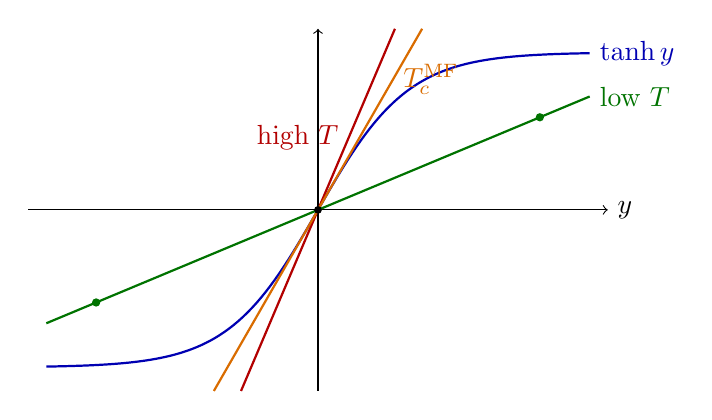
\begin{tikzpicture}[x=1.15cm,y=2.0cm]
\draw[->] (-3.2,0) -- (3.2,0) node[right] {$y$};
\draw[->] (0,-1.15) -- (0,1.15);
\draw[thick,blue!70!black,domain=-3:3,samples=120]
  plot (\x,{tanh(\x)}) node[right] {$\tanh y$};
\draw[thick,red!70!black] (-0.85,-1.15) -- (0.85,1.15)
  node[pos=0.70,left] {high \(T\)};
\draw[thick,orange!85!black] (-1.15,-1.15) -- (1.15,1.15)
  node[pos=0.86,right] {\(T_c^{\rm MF}\)};
\draw[thick,green!45!black] (-3,-0.72) -- (3,0.72)
  node[right] {low \(T\)};
\fill (0,0) circle (1.4pt);
\fill[green!45!black] (-2.45,-0.588) circle (1.5pt);
\fill[green!45!black] (2.45,0.588) circle (1.5pt);
\end{tikzpicture}
\caption{A normalized reconstruction of the graphical self-consistency argument.}
\end{figure}

The nonzero branch emerges continuously. Near the transition,
\begin{equation}
\tanh(Km)=Km-\frac{(Km)^3}{3}+O(m^5).
\end{equation}
For \(K>1\), the small nonzero solutions satisfy
\begin{equation}
m^2\simeq \frac{3(K-1)}{K^3}.
\end{equation}
Thus mean field predicts the familiar square-root onset \(m\propto(T_c-T)^{1/2}\).

The stability statement can also be made without relying on how the graph is drawn. Up to an \(m\)-independent constant, the mean-field free energy per spin is
\begin{equation}
f_{\rm MF}(m)
=dJm^2-\frac{1}{\beta}
\log\!\left[2\cosh(2\beta dJm)\right].
\label{eq:mf-free-energy}
\end{equation}
Its stationary condition is
\begin{equation}
\frac{\partial f_{\rm MF}}{\partial m}
=2dJ\left[m-\tanh(2\beta dJm)\right]=0.
\end{equation}
Above \(T_c^{\rm MF}\), \(m=0\) is the minimum. Below it, the origin is a local maximum and the two nonzero solutions are degenerate minima. The geometry of the intersections and the thermodynamics of the free energy say the same thing.

\begin{classroomqa}
\audiencequestion{The solution \(m=0\) remains an intersection below \(T_c^{\rm MF}\). Why should the nonzero branch be physical?}
\lecturerresponse{Following the system upward from zero temperature already places it on a magnetized branch. More formally, the mean-field free energy has minima at \(\pm m_0\) below the transition, while \(m=0\) becomes a maximum. An infinitesimal external field then selects one minimum and removes the apparent ambiguity. \lecturetimestamp{01:11:34--01:12:18}}
\end{classroomqa}

\section{Why One Dimension Defeats Mean Field}

Substituting \(d=1\) into Equation~\eqref{eq:mean-field-tc} would predict a transition at \(T=2J\), contradicting the exact one-dimensional solution. Nothing algebraic blows up. The approximation fails because two neighbors are not a large statistical bath, and because one-dimensional domain walls carry an exceptional entropy.

Start from the all-up state. A broken bond changes its energy from \(-J\) to \(+J\), so each broken bond costs
\begin{equation}
\Delta E_{\rm bond}=2J.
\end{equation}
On a square lattice, one flipped spin breaks four bonds and costs \(8J\). Two adjacent flipped spins have a perimeter of six broken bonds and cost \(12J\), whereas two far-separated flips break eight bonds and cost \(16J\).

\begin{figure}[ht]
\centering

\includegraphics[width=0.82\textwidth]{lecture_09_figure_09.png}
\caption{Two adjacent reversed spins in a square lattice; their shared bond is satisfied, leaving a six-bond boundary.}
\lectureframe{01:17:30}
\end{figure}

In two dimensions a compact reversed droplet therefore pays an energy proportional to its boundary length:
\begin{equation}
\Delta E_{\rm 2d}=2J\,|\partial D|.
\end{equation}
Growing the droplet generally grows its boundary.

One dimension is different. A contiguous reversed block, no matter how long, has only two domain walls:
\begin{equation}
\Delta E_{\rm 1d}=2(2J)=4J.
\label{eq:one-d-domain-cost}
\end{equation}

\begin{figure}[ht]
\centering

\includegraphics[width=0.82\textwidth]{lecture_09_figure_10.png}
\caption{A long reversed block in one dimension bounded by only two domain walls.}
\lectureframe{01:19:10}
\end{figure}

There are of order \(N^2\) ways to choose the two walls of such a block in a chain of \(N\) sites. Their energy does not grow with the separation between the walls. At any positive temperature, entropy therefore supplies arbitrarily large reversed domains. In two dimensions the boundary energy can defeat the contour entropy at sufficiently low temperature. This energy-entropy competition is the geometric fact that mean field cannot see when it treats \(d=1\) and \(d=2\) merely as different numerical values of the same coefficient.

\begin{classroomqa}
\audiencequestion{Does the constant two-wall cost require the flipped spins to be adjacent?}
\lecturerresponse{Yes. The claim concerns one contiguous reversed block. If the flipped spins form several separated blocks, each block introduces two additional domain walls. The important point is that a single block can be arbitrarily long while retaining only two walls. \lecturetimestamp{01:18:32--01:18:40}}
\end{classroomqa}

\begin{classroomqa}
\audiencequestion{The mean-field equation itself seems to show no qualitative distinction between \(d=1\) and \(d=2\). Is that the problem?}
\lecturerresponse{Exactly. Mean field predicts a transition for every positive \(d\), so it is qualitatively wrong in one dimension. Its derivation assumed many weakly fluctuating neighbors and discarded domain-wall geometry. The exact bond solution, not the mean-field substitution \(d=1\), decides the one-dimensional case. \lecturetimestamp{01:19:44--01:20:28}}
\end{classroomqa}

\section{An External Field Selects the Phase}

Add a uniform field \(h\) with the convention that \(h>0\) favors \(\sigma=+1\):
\begin{equation}
H=-J\sum_{\langle ij\rangle}\sigma_i\sigma_j
-h\sum_i\sigma_i.
\label{eq:ising-with-field}
\end{equation}
The mean-field energy of one selected spin is
\begin{equation}
E_i^{\rm MF}=-(2dJm+h)\sigma_i,
\end{equation}
and the self-consistency equation becomes
\begin{equation}
\boxed{m=\tanh\!\left[\beta(2dJm+h)\right]}.
\label{eq:self-consistency-field}
\end{equation}
With \(K=2\beta dJ\) and \(y=Km\),
\begin{equation}
\frac{y}{K}=\tanh(y+\beta h).
\label{eq:shifted-graph}
\end{equation}

\begin{figure}[ht]
\centering

\includegraphics[width=0.82\textwidth]{lecture_09_figure_11.png}
\caption{The external-field term added to the self-consistency equation, together with the shifted graphical construction.}
\lectureframe{01:26:20}
\end{figure}

\begin{classroomqa}
\audiencequestion{Why is the field added only inside the hyperbolic tangent? Should it also alter the left side?}
\lecturerresponse{The left side is the assumed magnetization \(m\), or equivalently \(y/K\). The right side is the magnetization calculated for a spin in the total effective field \(2dJm+h\). Self-consistency sets those two quantities equal. Keeping \(y=Km\) fixed as the definition puts the new term only in the argument \(\tanh(y+\beta h)\). \lecturetimestamp{01:23:46--01:26:18}}
\end{classroomqa}

\begin{classroomqa}
\audiencequestion{Can the same graphical change be described by moving the straight lines rather than shifting the \(\tanh\) curve?}
\lecturerresponse{Yes. One may keep \(\tanh y\) fixed and rewrite the equation so that the straight line has a nonzero intercept. The intersections are identical. The two descriptions differ only in which side of the equation is chosen as the fixed graph. \lecturetimestamp{01:35:07--01:36:26}}
\end{classroomqa}

For \(h\neq0\), the origin is no longer a solution. Below \(T_c^{\rm MF}\), an arbitrarily small positive field selects the positive branch; a negative field selects the negative branch.

\begin{figure}[ht]
\centering

\includegraphics[width=0.82\textwidth]{lecture_09_figure_12.png}
\caption{A weak field removes the symmetric intersection and selects one magnetized branch.}
\lectureframe{01:36:22}
\end{figure}

The proper statement requires an order of limits. A finite system at exactly \(h=0\) has spin-flip symmetry and therefore \(\expect{m}=0\) in the full equilibrium ensemble. Spontaneous magnetization is
\begin{equation}
m_{\rm sp}
=\lim_{h\to0^+}\lim_{N\to\infty}\expect{m}_{N,h},
\end{equation}
with the thermodynamic limit taken first. Reversing the sign of the infinitesimal field gives \(-m_{\rm sp}\). The total field-energy difference is proportional to \(Nh\), so even a tiny field becomes decisive for a macroscopic sample.

The corresponding free energy makes the tilt visible:
\begin{equation}
f_{\rm MF}(m;h)
=dJm^2-\frac{1}{\beta}
\log\!\left[2\cosh\!\left(\beta(2dJm+h)\right)\right].
\end{equation}
At \(h=0\) the two wells are equally deep. A positive \(h\) lowers the positive-\(m\) well and raises the negative-\(m\) well. The perturbation per spin can be tiny while the total preference, multiplied by \(N\), is macroscopic.

\begin{classroomqa}
\audiencequestion{If the external field remains present, is the magnetization really spontaneous?}
\lecturerresponse{The field is used only to select a branch. At fixed \(T<T_c\), take the system to infinite size and then let \(h\to0^+\). The magnetization remains finite even though the selecting field vanishes. Reversing the limiting sign selects the opposite phase. \lecturetimestamp{01:33:15--01:34:18}}
\end{classroomqa}

\begin{classroomqa}
\audiencequestion{Is the zero-average solution actually impossible below the transition, or merely unstable?}
\lecturerresponse{At exactly zero field, a symmetric finite-volume ensemble with equal weight on the two orientations is possible and has average zero. What fails is its stability as a single macroscopic phase. An arbitrarily small field changes the extensive energy balance and selects one orientation; after the thermodynamic limit, the selected magnetization survives as the field is removed. \lecturetimestamp{01:34:25--01:35:06}}
\end{classroomqa}

\begin{classroomqa}
\audiencequestion{What happens to the field-biased solution at infinite temperature?}
\lecturerresponse{For fixed finite \(h\), both \(K=2\beta dJ\) and \(\beta h\) vanish as \(T\to\infty\). Equation~\eqref{eq:self-consistency-field} then gives \(m\to0\). The weak field selects a low-temperature branch, but it cannot maintain order against infinite thermal agitation. \lecturetimestamp{01:27:39--01:29:51}}
\end{classroomqa}

\begin{classroomqa}
\audiencequestion{As temperature and the graph shift are varied together, how can one be sure where the intersection goes?}
\lecturerresponse{The implicit equation is safer than the moving sketch. At low temperature and positive \(h\), its stable solution approaches \(m=+1\). At high temperature, expansion of the tangent gives
\[
m\simeq \beta(2dJm+h)
\quad\Longrightarrow\quad
m\simeq \frac{\beta h}{1-2\beta dJ},
\]
which tends to zero when \(\beta\to0\). The stable branch therefore connects the aligned low-temperature limit to the weakly polarized high-temperature limit without remaining at the unstable origin below the transition. \lecturetimestamp{01:29:53--01:33:04}}
\end{classroomqa}

\section{A Magnetic Reversal Is a Different Problem}

\begin{classroomqa}
\audiencequestion{What makes Earth's magnetic field reverse direction?}
\lecturerresponse{That question lies outside the equilibrium Ising model. Earth's main field is generated by the geodynamo: convection and rotation of electrically conducting fluid in the outer core sustain electric currents and magnetic field. Reversals are irregular reorganizations of that nonlinear dynamo, not a simple ferromagnetic domain flip in solid iron. Their detailed timing is not captured by one equilibrium order parameter, so the honest answer here is that the Ising calculation does not explain the trigger. The useful connection is only the general one: a system with two opposite large-scale orientations can undergo an instability between them.\footnote{See the \href{https://science.nasa.gov/science-research/earth-science/earths-magnetosphere-protecting-our-planet-from-harmful-space-energy/}{NASA overview of the geodynamo} and the \href{https://www.usgs.gov/programs/geomagnetism/introduction-geomagnetism}{USGS introduction to geomagnetism}.} \lecturetimestamp{01:38:39--01:40:32}}
\end{classroomqa}

The exact chain and the mean-field lattice now give two sharply different answers. In one dimension,
\begin{equation}
\expect{\sigma_i\sigma_{i+r}}
=\left[\tanh(\beta J)\right]^r
\longrightarrow0
\qquad (T>0),
\end{equation}
because finite-energy domain walls can separate arbitrarily long reversed intervals. With many neighbors, the self-consistent field instead admits stable nonzero solutions below
\begin{equation}
T_c^{\rm MF}=2dJ.
\end{equation}
The contrast is not merely algebraic. It is the competition among geometry, energy, entropy, and redundancy: whether an error can spread freely or whether the surrounding lattice can correct it.
